\documentclass[twoside]{article}
\usepackage[utf8]{inputenc}
\usepackage[ngerman]{babel}
\usepackage{libertine}
\usepackage[a4paper]{geometry}
\usepackage[dvipsnames]{xcolor}
\usepackage{pdfpages}
\usepackage{parskip}
\usepackage{amsmath, amsthm, amssymb, commath, mathtools}
\usepackage{cancel}
\usepackage{physics}
\usepackage{nicefrac}
\usepackage{booktabs}
\usepackage{tabularx}
\usepackage{tabu}
\usepackage{enumitem}
\usepackage{graphicx}
\graphicspath{{./plots/}{./images/}}
\usepackage{wrapfig}
\usepackage{caption}
\usepackage{float}
\usepackage{minted}
\usepackage{appendix}
\usepackage{icomma}
\usepackage{multirow}
\usepackage{multicol}
\usepackage{footmisc}
\usepackage[separate-uncertainty=true]{siunitx}
\sisetup{locale = DE}
\usepackage{circledsteps}

\usepackage{csquotes}
\MakeOuterQuote{"}
\renewcommand{\ttdefault}{cmtt}

\usepackage[colorlinks]{hyperref}
\usepackage{bookmark}
% https://tex.stackexchange.com/a/33701
\makeatletter
    \newcommand{\nonum}[0]{%
        \let\@oldseccntformat\@seccntformat %
        \renewcommand\@seccntformat[1]{}%
        }
    \newcommand{\resnum}[0]{\let\@seccntformat\@oldseccntformat}
\makeatother

\usepackage{chngcntr}
\counterwithin{figure}{section}

\newcommand{\versuch}[0]{MAG}
\newcommand{\versuchLang}[0]{Magnetisches Feld}

\hypersetup{
	pdftitle={P2 -- \versuch{} Auswertung},
	pdfauthor={Yudong Sun},
	bookmarksnumbered=true,
	bookmarksopen=true,
	bookmarksopenlevel=2,
	pdfstartview=Fit,
	pdfpagemode=UseOutlines,
	colorlinks=true,
	linkcolor=MidnightBlue,
	filecolor=magenta, 
	urlcolor=blue
}
\urlstyle{same}

\title{\versuch{} -- \versuchLang \\ Auswertung}
\author{Yudong Sun\\Gruppe F2-2}

\usepackage{fancyhdr}
\pagestyle{fancy}
\fancyhf{}
\fancyhead[RO]{Yudong Sun}
\fancyhead[LO]{Auswertung -- \versuch}
\fancyhead[LE]{Yudong Sun}
\fancyhead[RE]{Auswertung -- \versuch}
\cfoot{\thepage}

% Custom Defs
\newcommand*{\ra}[1]{\renewcommand{\arraystretch}{#1}}
\newcommand*{\maxi}[1]{\text{max}\left(#1\right)}
\newcommand*{\mini}[1]{\text{min}\left(#1\right)}
\newcommand*{\todo}[1]{\textcolor{red}{TODO: #1}}
\newcommand*{\iu}[1]{\textit{\underline{#1}}}
\newcommand*{\gnuplot}[0]{\texttt{gnuplot}}
\newcommand*{\captionbr}[0]{\\\rule{\textwidth}{0pt}\\\vspace{-\baselineskip}}
\newcommand*{\sigfig}[1]{\hspace{0.5cm}\text{(#1 sig. Zif.)}}
\newcommand*{\pbrace}[1]{\left(#1\right)}
\newcommand*{\sbrace}[1]{\left[#1\right]}
\newcommand*{\bDelta}[1]{\pbrace{\Delta #1}}
\newcommand*{\overbar}[1]{\overline{\raisebox{0pt}[1.2\height]{$#1$}}} % https://tex.stackexchange.com/a/87615

% \addto\captionsngerman{
%     \let\oldfigname\figurename
%     \renewcommand{\figurename}{[\oldfigname}
%     \let\oldthefig\thefigure
%     \renewcommand{\thefigure}{\oldthefig]}
% } % https://tex.stackexchange.com/a/17490
% https://tex.stackexchange.com/a/101624 new line in caption

% Gaußsche Fehler Erzeuger
\makeatletter
    \newcommand{\gausserror}[2]{% \gausserror{G}{faktoren}
        \sqrt{%
            \@tempswafalse
            \@for\factor:=#2
            \do{
                \if@tempswa+%
                \else%
                    \@tempswatrue%
                \fi%
                \left(\pdv{#1}{\factor}\Delta\factor\right)^2%
            }%
        }
    }
\makeatother
% https://tex.stackexchange.com/a/59912
% https://riptutorial.com/latex/example/28657/loops---repeating-things

% Add quad
\makeatletter
    \newcommand{\addquad}[1]{% \gausserror{G}{faktoren}
        \sqrt{%
            \@tempswafalse
            \@for\factor:=#1
            \do{
                \if@tempswa+%
                \else%
                    \@tempswatrue%
                \fi%
                \left(\Delta\factor\right)^2%
            }%
        }
    }
\makeatother

% Add quad
\makeatletter
    \newcommand{\addquadpure}[1]{% \gausserror{G}{faktoren}
        \sqrt{%
            \@tempswafalse
            \@for\factor:=#1
            \do{
                \if@tempswa+%
                \else%
                    \@tempswatrue%
                \fi%
                \left(\factor\right)^2%
            }%
        }
    }
\makeatother

% rej quad
\makeatletter
    \newcommand{\relquad}[1]{% \gausserror{G}{faktoren}
        \sqrt{%
            \@tempswafalse
            \@for\factor:=#1
            \do{
                \if@tempswa+%
                \else%
                    \@tempswatrue%
                \fi%
                \left(\frac{\Delta\factor}{\factor}\right)^2%
            }%
        }
    }
\makeatother

% / Custom Defs

\begin{document}

\maketitle

% Einstellungen
\nonum
\numberwithin{equation}{section}
% / Einstellungen

\section{Teilversuch 1: Basisbedienelemente des Oszilloskops}
	Die Positionseinstellungen \texttt{[Y-POS.I]} und \texttt{[Y-POS.II]} verschiebt die Kurve vertikal im Bildschirm des Oszilloskops. Die Positionseinstellungen \texttt{[X-POS.]} verschiebt die Kurve horizontal im Bildschirm des Oszilloskops. 

	Die Ablenkfaktoren \texttt{[VOLTS/DIV.]} bzw. \texttt{[TIME/DIV.]} vergrößert und verkleinert die dargestellte Kurve in die vertikale bzw. horizontale Richtung. Ob es verkleinert oder vergrößert werden, kommt darauf an, in welcher Richtung sie gedreht sind. 

	Mit diesen zwei Einstellungen kann man die Kurve auf dem Bildschirm beliebig darstellen. Mit Hilfe von \texttt{AUTOSET} sind diese Einstellungen automatisch gestellt, sodass man leicht eine vernünftige Kurve erhaltet. 

	Der Trigger ist eine Einstellung für die Spannungswert, an dem das "Sweep" (Zeitablenkung) anfängt. Damit kann man ein periodisches Signal statisch im Bildschirm darstellen, sodass Messungen gemacht werden kann. Mit dem \texttt{[Level]} Knopf kann man diesen Spannungswert ändern, sodass die Kurve am verschiedene Zeitpunkten anfängt. Man kann auch damit die Aufnahme bei einem ganz bestimmten Punkt eines nicht-periodischen Signals anfangen, was sehr hilfreich sein kann. 
\newpage
\section{Teilversuch 2: Drehmoment des Feldes auf eine stromdurchflossene Spule}
	Fehler bei der Winkelmessung $\Delta \alpha = \SI{2}{\degree}$ \\
	Fehler bei der Winkelmessung $\Delta \beta = \SI{1.0}{\degree}$
 	\begin{equation*}
 		\begin{tabu}{l *{10}{l}}
 			\toprule
 			\alpha / \si{\degree} & 0 & 10 & 20 & 30 & 40 & 50 & 60 & 70 & 80 & 90 \\
 			\midrule
			\beta/ \si{\degree} & 295,0 & 315,0 & 337,0 & 358,5 & 377,0 & 395,0 & 413,0 & 425,5 & 437,5 & 449,0 \\
			(\beta - \beta_0)/ \si{\degree} & 0,0 & 20,0 & 42,0 & 63,5 & 82,0 & 100,0 & 118,0 & 130,5 & 142,5 & 154,0 \\
			\varphi / \si{\degree} & 0,0 & -10,0 & -22,0 & -33,5 & -42,0 & -50,0 & -58,0 & -60,5 & -62,5 & -64,0 \\
			\bottomrule
 		\end{tabu}
 	\end{equation*}
	wobei $\varphi = \alpha - (\beta - \beta_0)$.

	$\varphi$ wurde dann gegen $\sin (\alpha/\si{\degree})$ im \gnuplot{} geplottet und eine Kurveanpassung zur $\varphi = m\sin \alpha + c$ durchgeführt. 
	\begin{figure}[H]
		\centering
		% GNUPLOT: LaTeX picture with Postscript
\begingroup
  \makeatletter
  \providecommand\color[2][]{%
    \GenericError{(gnuplot) \space\space\space\@spaces}{%
      Package color not loaded in conjunction with
      terminal option `colourtext'%
    }{See the gnuplot documentation for explanation.%
    }{Either use 'blacktext' in gnuplot or load the package
      color.sty in LaTeX.}%
    \renewcommand\color[2][]{}%
  }%
  \providecommand\includegraphics[2][]{%
    \GenericError{(gnuplot) \space\space\space\@spaces}{%
      Package graphicx or graphics not loaded%
    }{See the gnuplot documentation for explanation.%
    }{The gnuplot epslatex terminal needs graphicx.sty or graphics.sty.}%
    \renewcommand\includegraphics[2][]{}%
  }%
  \providecommand\rotatebox[2]{#2}%
  \@ifundefined{ifGPcolor}{%
    \newif\ifGPcolor
    \GPcolortrue
  }{}%
  \@ifundefined{ifGPblacktext}{%
    \newif\ifGPblacktext
    \GPblacktexttrue
  }{}%
  % define a \g@addto@macro without @ in the name:
  \let\gplgaddtomacro\g@addto@macro
  % define empty templates for all commands taking text:
  \gdef\gplbacktext{}%
  \gdef\gplfronttext{}%
  \makeatother
  \ifGPblacktext
    % no textcolor at all
    \def\colorrgb#1{}%
    \def\colorgray#1{}%
  \else
    % gray or color?
    \ifGPcolor
      \def\colorrgb#1{\color[rgb]{#1}}%
      \def\colorgray#1{\color[gray]{#1}}%
      \expandafter\def\csname LTw\endcsname{\color{white}}%
      \expandafter\def\csname LTb\endcsname{\color{black}}%
      \expandafter\def\csname LTa\endcsname{\color{black}}%
      \expandafter\def\csname LT0\endcsname{\color[rgb]{1,0,0}}%
      \expandafter\def\csname LT1\endcsname{\color[rgb]{0,1,0}}%
      \expandafter\def\csname LT2\endcsname{\color[rgb]{0,0,1}}%
      \expandafter\def\csname LT3\endcsname{\color[rgb]{1,0,1}}%
      \expandafter\def\csname LT4\endcsname{\color[rgb]{0,1,1}}%
      \expandafter\def\csname LT5\endcsname{\color[rgb]{1,1,0}}%
      \expandafter\def\csname LT6\endcsname{\color[rgb]{0,0,0}}%
      \expandafter\def\csname LT7\endcsname{\color[rgb]{1,0.3,0}}%
      \expandafter\def\csname LT8\endcsname{\color[rgb]{0.5,0.5,0.5}}%
    \else
      % gray
      \def\colorrgb#1{\color{black}}%
      \def\colorgray#1{\color[gray]{#1}}%
      \expandafter\def\csname LTw\endcsname{\color{white}}%
      \expandafter\def\csname LTb\endcsname{\color{black}}%
      \expandafter\def\csname LTa\endcsname{\color{black}}%
      \expandafter\def\csname LT0\endcsname{\color{black}}%
      \expandafter\def\csname LT1\endcsname{\color{black}}%
      \expandafter\def\csname LT2\endcsname{\color{black}}%
      \expandafter\def\csname LT3\endcsname{\color{black}}%
      \expandafter\def\csname LT4\endcsname{\color{black}}%
      \expandafter\def\csname LT5\endcsname{\color{black}}%
      \expandafter\def\csname LT6\endcsname{\color{black}}%
      \expandafter\def\csname LT7\endcsname{\color{black}}%
      \expandafter\def\csname LT8\endcsname{\color{black}}%
    \fi
  \fi
    \setlength{\unitlength}{0.0500bp}%
    \ifx\gptboxheight\undefined%
      \newlength{\gptboxheight}%
      \newlength{\gptboxwidth}%
      \newsavebox{\gptboxtext}%
    \fi%
    \setlength{\fboxrule}{0.5pt}%
    \setlength{\fboxsep}{1pt}%
\begin{picture}(8640.00,5760.00)%
    \gplgaddtomacro\gplbacktext{%
      \csname LTb\endcsname%%
      \put(682,704){\makebox(0,0)[r]{\strut{}$25$}}%
      \put(682,1192){\makebox(0,0)[r]{\strut{}$26$}}%
      \put(682,1681){\makebox(0,0)[r]{\strut{}$27$}}%
      \put(682,2169){\makebox(0,0)[r]{\strut{}$28$}}%
      \put(682,2657){\makebox(0,0)[r]{\strut{}$29$}}%
      \put(682,3146){\makebox(0,0)[r]{\strut{}$30$}}%
      \put(682,3634){\makebox(0,0)[r]{\strut{}$31$}}%
      \put(682,4122){\makebox(0,0)[r]{\strut{}$32$}}%
      \put(682,4611){\makebox(0,0)[r]{\strut{}$33$}}%
      \put(682,5099){\makebox(0,0)[r]{\strut{}$34$}}%
      \put(814,484){\makebox(0,0){\strut{}$-100$}}%
      \put(1489,484){\makebox(0,0){\strut{}$0$}}%
      \put(2165,484){\makebox(0,0){\strut{}$100$}}%
      \put(2840,484){\makebox(0,0){\strut{}$200$}}%
      \put(3515,484){\makebox(0,0){\strut{}$300$}}%
      \put(4191,484){\makebox(0,0){\strut{}$400$}}%
      \put(4866,484){\makebox(0,0){\strut{}$500$}}%
      \put(5542,484){\makebox(0,0){\strut{}$600$}}%
      \put(6217,484){\makebox(0,0){\strut{}$700$}}%
      \put(6892,484){\makebox(0,0){\strut{}$800$}}%
      \put(7568,484){\makebox(0,0){\strut{}$900$}}%
      \put(8243,484){\makebox(0,0){\strut{}$1000$}}%
    }%
    \gplgaddtomacro\gplfronttext{%
      \csname LTb\endcsname%%
      \put(209,2901){\rotatebox{-270}{\makebox(0,0){\strut{}Temperatur $\theta$ ($\si{\celsius}$)}}}%
      \put(4528,154){\makebox(0,0){\strut{}Zeit $t$ ($\si{\second}$)}}%
      \csname LTb\endcsname%%
      \put(946,4893){\makebox(0,0)[l]{\strut{}$0,00832t + 25,66397$}}%
      \csname LTb\endcsname%%
      \put(946,4607){\makebox(0,0)[l]{\strut{}Messpunkte}}%
      \csname LTb\endcsname%%
      \put(4528,5429){\makebox(0,0){\strut{}Erwärmung von Wasser im Kalorimeter}}%
    }%
    \gplbacktext
    \put(0,0){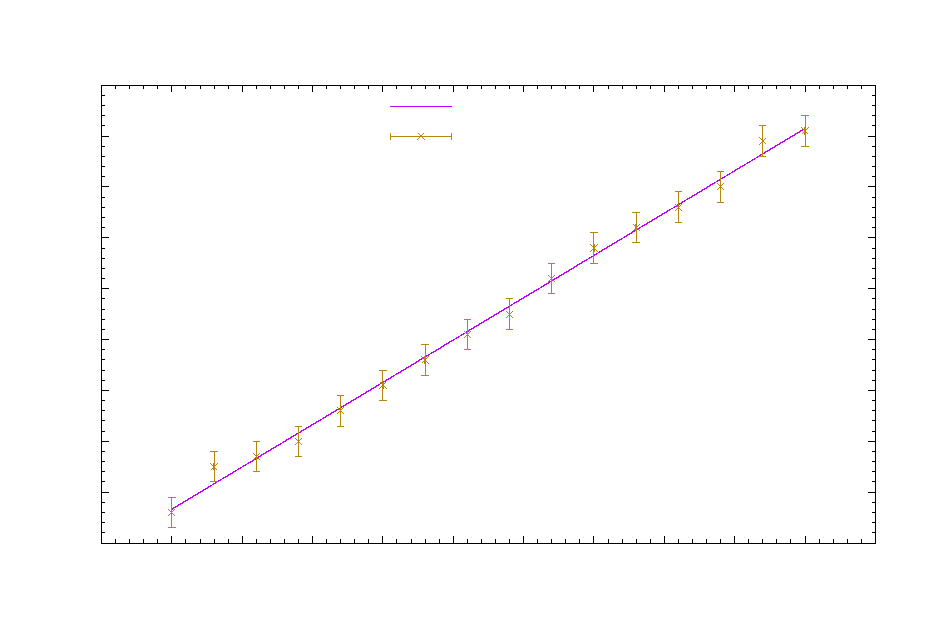
\includegraphics[width={432.00bp},height={288.00bp}]{tv1-plot}}%
    \gplfronttext
  \end{picture}%
\endgroup

		\caption{\centering Drehmoment auf stromdurchflossene Spule \captionbr $\chi^2_{\text{red}} = \num{0.0525026} \implies$ Gute Anpassung}
		\label{fig:tvone-plot}
		\vspace{-1em}
	\end{figure}

\newpage
\section{Teilversuch 3: Bestimmung der spezifischen Schmelzwärme von Eis}
Wir berechnen zunächst die Masse von Wasser und Eis, die im Experiment verwendet wurden:
\begin{align}
	m_1 &= m_\text{wasser} = m_\text{Wasser+Alu} - m_\text{Alu} =\SI{717.30}{\gram} - \SI{295.06}{\gram} = \SI{422.24}{\gram} \\
	\Delta m_1 &= \sqrt{(\Delta m_\text{Wasser+Alu})^2 + (\Delta m_\text{Alu})^2} = \sqrt{(\SI{0.13}{\gram})^2 + (\SI{0.03}{\gram})^2} \notag \\
	&= \SI{0.14}{\gram} \\
	m_\text{Eis} &= m_\text{Eis+Alu} - m_\text{Alu} =\SI{505.14}{\gram} - \SI{296.65}{\gram} = \SI{208.49}{\gram} \\
	\Delta m_\text{Eis} &= \sqrt{(\Delta m_\text{Eis+Alu})^2 + (\Delta m_\text{Alu})^2} = \sqrt{(\SI{0.03}{\gram})^2 + (\SI{0.03}{\gram})^2} \notag \\
	&= \SI{0.05}{\gram} \\
\end{align}
Aus der Anleitung gilt:
\begin{align}
	c_\text{w} m_{\text{Eis}}(T_M-T_0) + \lambda m_{\text{Eis}} &= c_\text{w}(m_1 + m_w^*) (T_1 - T_M) \\
	\Leftrightarrow  \lambda &= \frac{c_\text{w} \left[(m_1 + m_w^*)(T_1 -T_M) - m_\text{Eis} (T_M -T_0)\right] }{m_\text{Eis}} \notag \\
	&=\frac{c_\text{w}}{m_\text{Eis}}(m_1 + m_w^*)(T_1 -T_M) - c_\text{w}(T_M -T_0)
\end{align}
mit dem Fehler:
\begin{align}
	\Delta \lambda = \gausserror{\lambda}{m_1, T_1, T_M, T_0, m_\text{Eis}, m_w^*}
\end{align}
wobei:
\begin{align*}
	\pdv{\lambda}{m_1} &= \frac{c_\text{w}}{m_\text{Eis}}(T_1 - T_M) = \pdv{\lambda}{m_w^*} \\
	\pdv{\lambda}{T_1} &= \frac{c_\text{w}}{m_\text{Eis}}(m_1 + m_w^*) \\
	\pdv{\lambda}{T_m} &= -\frac{c_\text{w}}{m_\text{Eis}}(m_1 + m_w^*) - c_\text{w} \\
	\pdv{\lambda}{T_0} &= c_\text{w} \\
	\pdv{\lambda}{m_\text{Eis}} &= \frac{c_\text{w}}{m^2_\text{Eis}}(m_1 + m_w^*)(T_1 -T_M)
\end{align*}
somit:
\begin{align*}
	\Delta \lambda &= \left[
		\left(\frac{c_\text{w}}{m_\text{Eis}}(T_1 - T_M) \Delta m_1\right)^2 
		+ \left(\frac{c_\text{w}}{m_\text{Eis}}(m_1 + m_w^*) \Delta T_1\right)^2
		+ \left(\left(-\frac{c_\text{w}}{m_\text{Eis}}(m_1 + m_w^*) - c_\text{w}\right) \Delta T_m\right)^2 \right. \\
		&\phantom{=} \left. + \left(c_\text{w} \Delta T_0\right)^2 
		+ \left(\frac{c_\text{w}}{m^2_\text{Eis}}(m_1 + m_w^*)(T_1 -T_M) \Delta m_\text{Eis}\right)^2 
		+ \left(\frac{c_\text{w}}{m_\text{Eis}}(T_1 - T_M) \Delta m_w^*\right)^2
	\right]^{1/2}
\end{align*}
% Wir benutzen im diesem Fall den von Hersteller gegebenen Wasserwert, somit verschwinden auch die Unsicherheit in dem Wasserwert. 
\newpage
Mit der Werten:
\begin{center}
	\begin{tabular}{lll}
		\toprule
		Variable & Wert & Bedeutung \\
		\midrule
		$m_1$ & \SI{422.24(14)}{\gram} & Masse des Wassers \\
		$m_\text{Eis}$ & \SI{208.49(5)}{\gram} & Masse des Eises \\
		$m_w^*$ & \SI{50(30)}{\gram} & Wasserwert des Kalorimeters \\
		$T_1$ & \SI{47.8(1)}{\celsius} & Temperatur des Wassers \\
		$T_M$ & \SI{16.8(2)}{\celsius} & Temperatur des Mischung \\
		$T_0$ & \SI{1.5(1)}{\celsius} & Temperatur des Eises \\
		$c_\text{w}$ & \SI{4.18}{\joule\per\gram\per\kelvin} & Spezifische Wärmekapazität des Wassers\\
		\bottomrule
	\end{tabular}
\end{center}
haben wir:
\begin{align*}
	\lambda &= \frac{\SI{4.18}{\joule\per\gram\per\kelvin}}{\SI{208.49}{\gram}}(\SI{422.24}{\gram} + \SI{80}{\gram})(\SI{47.8}{\celsius} -\SI{16.8}{\celsius}) - (\SI{4.18}{\joule\per\gram\per\kelvin})(\SI{16.8}{\celsius} -\SI{1.5}{\celsius}) \\
	&= \SI{229.551}{\joule\per\gram} \sigfig{6} \\
	\Delta \lambda &= \SI{18.8730}{\joule\per\gram} \sigfig{6} \\
	\Rightarrow \lambda &= \SI{230(19)}{\joule\per\gram}
\end{align*}
Sodass die Ergebnisse überschaubar bleiben, sind die Subtitution hier nicht explizit hingeschrieben.

Im Vergleich zum Literaturwert von $\SI{333}{\joule\per\gram}$ unterscheidet sich die zwei Werten signifikant voneinander. Diese Unterschied könnte daran liegen, dass die Masse von dem benutzten Eis schwer bestimmbar ist. Es gibt oft immer noch ein bisschen geschmolzte Eis (Wasser), ob wir das Tauwasser schon gegossen haben. Das soll zu einer größeren Unsicherheit bei der Masse der Eis führen, was in diesem Fall nicht berücksichtigt geworden ist. Mit weniger Eis, wird die Temperaturunterschied $(T_1 - T_M)$ kleiner sein, was weiter zu einer niedriger Schmelzwärme führen wird.

Es ist auch beobachtet, dass die Temperatur des Eises nicht $\SI{0}{\celsius}$ ist. Das könnte entweder aus einem Fehler im Thermometer entstehen, oder es gibt Verunreinigungen im Eis, was die Schmelzwärme ändern werden. Außerdem könnte es auch noch Wärmeaustausch mit der Umgebung geben, was schwer zu messen ist. Alle diese Gründe werden zu einer niedriger Schmelzwärme führen, was hier erhalten ist. 
\section{Teilversuch 4: Induktion durch ein zeitlich veränderliches Magnetfeld}

\resnum
\newpage
\appendix
\section{Quellcode zur Auswertung von Teilversuch 1}
    \label{appdx:tvone}

    \gnuplot{} Quellcode für warmes Spülmittel
    {  
        % % Surpress "errors" in minted
        % https://tex.stackexchange.com/a/289068
        \renewcommand{\fcolorbox}[4][]{#4}
        \inputminted[linenos,breaklines,autogobble,frame=leftline,framesep=10pt]{gnuplot}{./plots/data-warm/process.gp}
    }
    \textattachfile[author={Yudong Sun},color={0 0.404 0.584},description={.zip Datei mit der Messwerten},mimetype={application/zip},timezone={+02'00'}]{./attachments/luftblasen-warm.zip}{Die Daten stehen als Anhang dieses PDF-Dokuments zur Verfügung.}}
\end{document}
